% CricShot shot-classification agent: architecture, explained simply.
% CricShot Day 44. Becomes CricketMind's classifier node (its Phase 8).
% No accuracy numbers on purpose: they belong to the CricShot accuracy
% paper only, and this agent will live inside CricketMind.

\documentclass[11pt,a4paper]{article}

\usepackage[margin=2cm]{geometry}
\usepackage[T1]{fontenc}
\usepackage[utf8]{inputenc}
\usepackage{lmodern}
\usepackage{booktabs}
\usepackage{array}
\usepackage{xcolor}
\usepackage{amsmath}
\usepackage{enumitem}
\usepackage{float}
\usepackage[font=small,labelfont=bf]{caption}
\usepackage{tikz}
\usetikzlibrary{shapes.geometric,arrows.meta,positioning,calc}
\usepackage[hidelinks]{hyperref}

\definecolor{prepblue}{RGB}{31,58,110}     % preparing the clip
\definecolor{gatered}{RGB}{170,30,40}      % decisions
\definecolor{fastteal}{RGB}{17,110,110}    % the fast model
\definecolor{expertgreen}{RGB}{27,94,58}   % the experts
\definecolor{fuseviolet}{RGB}{88,48,132}   % fusing and explaining
\definecolor{outgrey}{RGB}{45,45,50}       % input and output

\tikzset{
  step/.style={rectangle, rounded corners=3pt, draw=#1, very thick,
               fill=#1!8, text width=5.4cm, align=center,
               minimum height=1.05cm, font=\small},
  gate/.style={diamond, aspect=2.6, draw=gatered, very thick,
               fill=gatered!8, text width=2.4cm, align=center,
               inner sep=1pt, font=\small},
  expert/.style={rectangle, rounded corners=3pt, draw=expertgreen,
                 very thick, fill=expertgreen!8, text width=3.0cm,
                 align=center, minimum height=1.3cm, font=\footnotesize},
  io/.style={rectangle, draw=outgrey, very thick, fill=outgrey!6,
             text width=3.6cm, align=center, minimum height=0.9cm,
             font=\small},
  note/.style={rectangle, draw=prepblue, dashed, fill=white,
               text width=3.3cm, align=center, font=\footnotesize},
  arrow/.style={-{Stealth[length=2.6mm]}, thick},
  lab/.style={font=\footnotesize\itshape, fill=white, inner sep=1.5pt},
}

\newcommand{\why}[1]{\par\noindent\textbf{Why it is there:} #1}
\newcommand{\inout}[2]{\par\noindent\textbf{In:} #1 \quad
  \textbf{Out:} #2}

\title{\textbf{A Shot-Classification Agent for CricShot10k}\\[2pt]
  \large How it is built, explained simply}
\author{CricShot project}
\date{}

\begin{document}
\maketitle
\vspace{-6ex}

\section*{In one paragraph}

The agent watches one broadcast clip of a batter and says which of the 15
cricket shots it is. It first finds the batter and cuts out the frames
that matter. If it cannot see the batter well enough, it says so instead of
guessing. Otherwise one small, quick model gives an answer. If that model
is sure, the agent answers straight away. If it is not sure, several
bigger models that look at the clip in different ways are asked, and
their answers are combined by a weighted vote. The agent always explains
its answer: the top three shots, which models agreed, and the frames that
mattered.

Every step is an ordinary function around a trained model. There is no
large language model inside: the agent is a fixed flowchart, built with
LangGraph so it can plug into CricketMind as one node.
Figure~\ref{fig:agent} shows the whole agent.

\begin{figure}[H]
\centering
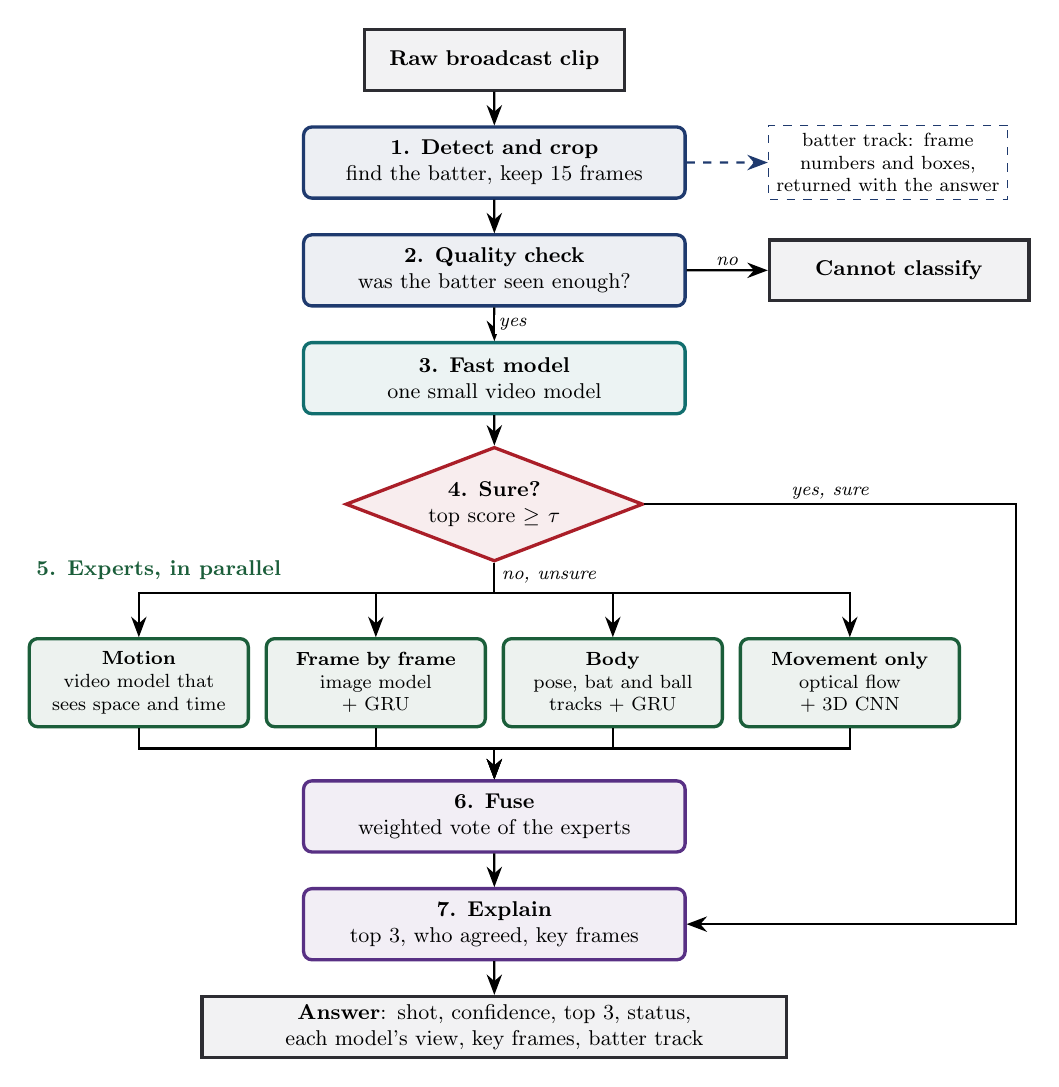
\begin{tikzpicture}[node distance=0.5cm, scale=0.86, transform shape]

  \coordinate (rail) at (7.7,0);

  \node[io] (clip) {\textbf{Raw broadcast clip}};
  \node[step=prepblue, below=of clip] (crop)
       {\textbf{1. Detect and crop}\\find the batter, keep 15 frames};
  \node[note, right=1.2cm of crop] (track)
       {batter track: frame numbers and boxes, returned with the answer};
  \node[step=prepblue, below=of crop] (quality)
       {\textbf{2. Quality check}\\was the batter seen enough?};
  \node[io, right=1.2cm of quality] (refuse) {\textbf{Cannot classify}};
  \node[step=fastteal, below=of quality] (fast)
       {\textbf{3. Fast model}\\one small video model};
  \node[gate, below=0.45cm of fast] (gate)
       {\textbf{4. Sure?}\\top score $\geq \tau$};

  \node[expert, anchor=north] (e1) at ($(gate.south)+(-5.25,-1.1)$)
       {\textbf{Motion}\\video model that\\sees space and time};
  \node[expert, anchor=north] (e2) at ($(gate.south)+(-1.75,-1.1)$)
       {\textbf{Frame by frame}\\image model\\+ GRU};
  \node[expert, anchor=north] (e3) at ($(gate.south)+(1.75,-1.1)$)
       {\textbf{Body}\\pose, bat and ball\\tracks + GRU};
  \node[expert, anchor=north] (e4) at ($(gate.south)+(5.25,-1.1)$)
       {\textbf{Movement only}\\optical flow\\+ 3D CNN};
  \node[font=\small\bfseries, text=expertgreen, anchor=south west]
       at ($(e1.north west)+(0,0.72)$) {5. Experts, in parallel};

  \node[step=fuseviolet, anchor=north] (fuse) at ($(gate.south)+(0,-3.2)$)
       {\textbf{6. Fuse}\\weighted vote of the experts};
  \node[step=fuseviolet, below=of fuse] (explain)
       {\textbf{7. Explain}\\top 3, who agreed, key frames};
  \node[io, below=of explain, text width=8.4cm] (answer)
       {\textbf{Answer}: shot, confidence, top 3, status,\\
        each model's view, key frames, batter track};

  \draw[arrow] (clip) -- (crop);
  \draw[arrow, dashed, prepblue] (crop) -- (track);
  \draw[arrow] (crop) -- (quality);
  \draw[arrow] (quality) -- node[lab, above] {no} (refuse);
  \draw[arrow] (quality) -- node[lab, right] {yes} (fast);
  \draw[arrow] (fast) -- (gate);
  \draw[arrow] (gate.east) -- node[lab, above, pos=0.5] {yes, sure}
       (gate.east -| rail) |- (explain.east);
  \foreach \e in {e1, e2, e3, e4} {
    \draw[arrow] (gate.south) -- ++(0,-0.45) -| (\e.north);
    \draw[arrow] (\e.south) -- ++(0,-0.3) -| (fuse.north);
  }
  \node[lab, right] at ($(gate.south)+(0.05,-0.22)$) {no, unsure};
  \draw[arrow] (fuse) -- (explain);
  \draw[arrow] (explain) -- (answer);
\end{tikzpicture}
\caption{The agent. Blue prepares the clip, red decides, teal is the one
quick model, green are the experts that are only asked when the quick
model is unsure, and violet combines and explains. A clip takes the short
path (1, 2, 3, 4, 7) whenever the quick model is sure.}
\label{fig:agent}
\end{figure}

\section{Each step, simply}

\subsection*{1. Detect and crop}
A detector (YOLO, trained by the CricShot10k authors) finds the batter in
every frame. Around the batter the agent cuts a square, so the batter fills
the picture and the crowd mostly does not. It keeps the main camera shot,
drops repeated frames, and picks 15 frames spread evenly over the stroke.
\inout{a raw video clip}{15 cropped frames of $224 \times 224$ pixels, and
the \emph{batter track}: for every kept frame, its number in the raw clip
and the box that was cut out}
\why{every model in CricShot was trained on frames made exactly this way.
Frames made any other way look different to the models, and they answer
worse without any error message. The batter track lets CricketMind run
its own pose measurements on the very same frames.}

\subsection*{2. Quality check}
If the batter was found in too few frames, the agent stops and returns
\emph{cannot classify}. It uses the same rule CricShot's preprocessing
uses to drop a clip.
\inout{the 15 frames and how often the batter was found}{go on, or stop}
\why{a confident guess about a clip with no batter in it is worse than an
honest ``I can't tell''.}

\subsection*{3. The fast model}
One small video model looks at the 15 frames and gives a score to each of
the 15 shots. The scores are turned into probabilities that add up to 1
(see Section~\ref{sec:maths}).
\inout{15 frames}{15 probabilities, one per shot}
\why{most clips are easy. A small model answers them quickly, so the big
models only run when they are needed.}
\par\noindent\textbf{Candidates from Phase 3:} X3D-M or R(2+1)D-18, both
small and quick. The final choice is made on validation data in Phase 4.

\subsection*{4. The confidence gate}
The agent looks at the fast model's highest probability. If it is at least
a threshold $\tau$ (for example $0.9$), the agent is sure and goes straight
to step 7. If not, it asks the experts.
\inout{15 probabilities}{``sure'' or ``unsure''}
\why{this is the agent's main decision: answer now, or spend more effort.
A higher $\tau$ means more clips go to the experts: slower, but more
careful.}

\subsection*{5. The experts}
Several stronger models each give their own 15 probabilities, all at the
same time. They are chosen because they look at the clip in different
ways:
\begin{itemize}[nosep, leftmargin=1.4em]
  \item \textbf{Motion:} a video model that sees space and time together
        (candidates: MViT-v2-S, SlowFast).
  \item \textbf{Frame by frame:} an image model describes each frame,
        and a GRU reads the 15 descriptions in order (ConvNeXt-T + GRU).
  \item \textbf{Body:} the batter's 33 body points, plus the bat's and the
        ball's paths, read by a GRU (pose GRU, or bat + ball + pose).
  \item \textbf{Movement only:} optical flow, how every pixel moved between
        frames, read by a 3D CNN (flow r3d\_18).
\end{itemize}
\inout{the 15 frames (and the pose and flow made from them)}{one set of 15
probabilities per expert}
\why{models that see differently make \emph{different} mistakes, so when
they vote, one model's mistake can be outvoted by the others. Phase 3
already found that averaging a body-pose model with a picture model beats
either one alone.}

\subsection*{6. Fuse}
The experts' probabilities are averaged, with a weight for each expert
(Section~\ref{sec:maths}). Better experts get bigger weights. The shot
with the highest combined probability is the answer.
\inout{one set of probabilities per expert}{one combined set}
\why{a weighted vote is simple, has very few numbers to learn, and so
cannot memorise the training clips. In Phase 3, a plain average beat a
fusion layer that had to be trained.}

\subsection*{7. Explain}
The agent writes down the top three shots with their probabilities, which
models agreed with the answer, and the frames that mattered most (from the
models' attention or from Grad-CAM heat maps).
\inout{the answer and every model's view}{a short explanation}
\why{an answer you can check is worth more than one you have to trust.
It also shows \emph{where} the agent is unsure, e.g.\ between a pull and
a hook.}

\section{The maths, simply}
\label{sec:maths}

\paragraph{Scores to probabilities.}
A model gives one score $s_c$ to each shot $c$. The softmax turns scores
into probabilities that are positive and add up to 1:
\[
  p(c) \;=\; \frac{e^{s_c}}{\sum_{k=1}^{15} e^{s_k}} .
\]
A higher score gives a higher probability.

\paragraph{Confidence.}
The confidence is simply the biggest probability, and the answer is the
shot that has it:
\[
  \text{confidence} = \max_c \, p(c), \qquad
  \text{answer} = \arg\max_c \, p(c).
\]

\paragraph{The gate.}
\[
  \text{go to the experts} \iff \max_c \, p_{\text{fast}}(c) < \tau .
\]

\paragraph{The weighted vote.}
With experts $1, \dots, K$ and weights $w_1, \dots, w_K$ that are
positive and add up to 1:
\[
  p_{\text{fused}}(c) \;=\; \sum_{k=1}^{K} w_k \, p_k(c),
  \qquad \sum_{k=1}^{K} w_k = 1 .
\]
If every weight is the same, this is a plain average.

\paragraph{The status.}
\[
  \text{status} =
  \begin{cases}
    \texttt{cannot\_classify} & \text{the batter was not seen enough,}\\
    \texttt{low\_confidence}  & \text{even the fused confidence is below } \tau,\\
    \texttt{ok}               & \text{otherwise.}
  \end{cases}
\]
A \texttt{low\_confidence} answer is still given, but it is marked, so
nobody mistakes it for a sure one.

\section{A worked example}

\noindent\emph{The numbers below are made up, only to show how the steps
fit together. They are not results.}

\begin{enumerate}[leftmargin=1.6em]
  \item A clip comes in. The batter is found in 14 of 15 frames, so the
        quality check passes.
  \item The fast model says: Cover Drive $0.62$, Straight Drive $0.21$,
        Lofted Offside $0.09$, \dots{} Its confidence is $0.62$.
  \item With $\tau = 0.9$, $0.62 < 0.9$: the agent is unsure and asks the
        four experts.
  \item The experts say Cover Drive with $0.71$, $0.55$, $0.48$ and
        $0.66$; two of them put Straight Drive second.
  \item With weights $0.4, 0.2, 0.2, 0.2$, the fused probability of Cover
        Drive is $0.4\times0.71 + 0.2\times(0.55+0.48+0.66) = 0.62$, the
        highest of the 15. That is still below $\tau$, so the answer is
        Cover Drive with status \texttt{low\_confidence}.
  \item The explanation: ``Cover Drive (0.62), then Straight Drive and
        Lofted Offside. All four experts agree on Cover Drive. The bat's
        path in frames 8 to 11 mattered most.''
\end{enumerate}

\section{How it is set up (all on validation data)}

Three things are chosen, and all of them on the validation set, never on
the test set:
\begin{enumerate}[nosep, leftmargin=1.6em]
  \item \textbf{Which models.} The fast model is the best small one; the
        experts are the best model from each \emph{different} way of
        seeing (motion, frame by frame, body, movement only).
  \item \textbf{The weights} $w_k$: the ones that give the best combined
        result on validation clips.
  \item \textbf{The threshold} $\tau$: the lowest one at which the agent
        is still as good as asking every expert every time. Lower $\tau$
        means fewer clips need the experts, so the agent is faster.
\end{enumerate}
The test set is used once, at the very end, to report how well the
finished agent works.

\section{What the agent returns}

\begin{table}[H]
\centering
\small
\begin{tabular}{>{\ttfamily}l p{11cm}}
\toprule
\normalfont\textbf{Field} & \textbf{What it holds} \\
\midrule
shot        & the answer: one of the 15 shots \\
confidence  & the probability of that shot \\
top3        & the three most likely shots, with probabilities \\
status      & \texttt{ok}, \texttt{low\_confidence} or \texttt{cannot\_classify} \\
models      & which models were asked, and what each one said \\
key\_frames & the frames that mattered most \\
track       & every kept frame's number in the raw clip and its crop box;
              the 15 used by the models are marked \\
\bottomrule
\end{tabular}
\caption{The agent's output, the same for every clip.}
\end{table}

\section{Why it is built this way}

\begin{itemize}[nosep, leftmargin=1.4em]
  \item \textbf{Fast on easy clips:} most clips stop at the fast model.
  \item \textbf{Careful on hard clips:} several different views vote.
  \item \textbf{Honest:} it refuses clips it cannot read, and marks answers
        it is not sure of.
  \item \textbf{Checkable:} every answer comes with its reasons.
  \item \textbf{Simple:} each step is a plain function around a trained
        model; there is nothing to prompt and nothing random in the
        decisions.
\end{itemize}

\section{Where it lives}

The agent is built in the CricShot project after its final phase, when
the models, the weights and $\tau$ are known. It is then handed to
CricketMind as one LangGraph subgraph, which becomes CricketMind's
classifier node. CricketMind gives it a raw clip and gets back the output
in the table above. CricketMind describes the agent's design, but never
reports its accuracy: those numbers belong to the CricShot accuracy paper.

\section*{Words used here}

\begin{description}[nosep, leftmargin=1.6em, font=\normalfont\bfseries]
  \item[Agent] a program that takes a sequence of steps and makes
        decisions between them; here, a fixed flowchart.
  \item[Node] one step in the flowchart.
  \item[LangGraph] a Python library for building such flowcharts.
  \item[YOLO] a fast object detector, used to find the batter.
  \item[GRU] a small network that reads a sequence (here, 15 frames) in
        order and remembers what it has seen.
  \item[3D CNN] a network that looks at a short video as a block of
        frames, so it sees motion directly.
  \item[Pose] the positions of 33 body points (shoulders, elbows, hips,
        knees, \dots) in each frame.
  \item[Optical flow] for every pixel, how far and in which direction it
        moved since the frame before.
  \item[Softmax] the formula that turns scores into probabilities.
  \item[Validation set] clips set aside to make choices with; the test set
        is kept for the final, honest measurement.
\end{description}

\end{document}
